\section{Results}
\label{sec:results}

\subsection{H1: coverage overlap and redundancy}

Every project had pairs above the 0.9 threshold, so each contributed 50 sampled pairs (\HOnePairs{} in total). Among them, \HOneShare{} were mutually non-dominated: each test killed at least one mutant the other did not (95\% CI \HOneLo{} to \HOneHi{}, clustered by project). H1 is \textbf{\HOneSupported}. A further \HOneOneWay{} of pairs were one-way: one test's kill set strictly contained the other's, so only one of the two tests could be removed without losing kills, and the coverage score does not say which. Only the remaining pairs had identical kill sets. Overall, \HOneAnyDiff{} of high-overlap pairs differed in what they detect.

The share varied widely between projects (Table~\ref{tab:h1}), from \HOneMinShare{} in \HOneMinProject{} to \HOneMaxShare{} in \HOneMaxProject{}. Pairs of parametrized cases of the same test function were non-dominated less often (\HOneSameFnShare{} of \HOneSameFnN{}) than pairs of distinct functions (\HOneDistinctFnShare{} of \HOneDistinctFnN{}), but both are far from zero.

Across both strata, coverage Jaccard and kill-set Jaccard are correlated (Spearman $\rho = \HOneRho$, $n = \HOneRhoN$ pairs with at least one kill; Figure~\ref{fig:h1}). Overlap is therefore a reasonable signal for \emph{where to look}, which is how the audit uses it, but at the top of the scale it does not reliably separate redundant pairs from complementary ones.

\begin{table}[t]
\centering\small
\begin{tabular}{lrrrrr}
\toprule
Project & Pairs & Non-dominated & 95\% CI & One-way & Identical \\
\midrule
attrs & 50 & 11 (22\%) & 13--35\% & 21 & 18 \\
more-itertools & 50 & 10 (20\%) & 11--33\% & 21 & 19 \\
dateutil & 50 & 27 (54\%) & 40--67\% & 15 & 8 \\
toolz & 50 & 25 (50\%) & 37--63\% & 15 & 10 \\
marshmallow & 50 & 9 (18\%) & 10--31\% & 24 & 17 \\
click & 50 & 29 (58\%) & 44--71\% & 17 & 4 \\
tomlkit & 50 & 5 (10\%) & 4--21\% & 21 & 24 \\
cachetools & 50 & 24 (48\%) & 35--61\% & 16 & 10 \\
\bottomrule
\end{tabular}
\caption{H1: test pairs with coverage Jaccard $\geq 0.9$. \emph{Non-dominated}: each test kills a mutant the other misses. \emph{One-way}: one kill set strictly contains the other. \emph{Identical}: equal kill sets (including both empty). Per-project intervals are Wilson 95\%.}
\label{tab:h1}
\end{table}


\begin{figure}[t]
\centering
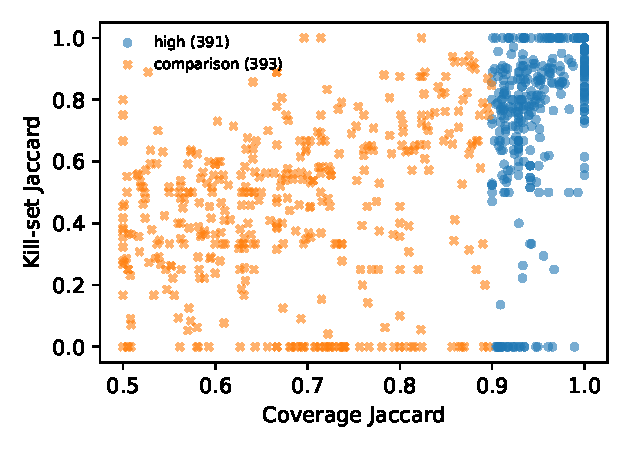
\includegraphics[width=0.6\linewidth]{figures/h1_scatter.pdf}
\caption{H1: coverage Jaccard against kill-set Jaccard for sampled pairs with at least one kill.}
\label{fig:h1}
\end{figure}

\subsection{H2: is deletion a cheaper way to find untested code?}

No. Under equal 20-minute wall-clock budgets, deletion mutants yielded \HTwoRatio{} times as many activated survivors per CPU-minute as mutmut's classical operators (95\% CI \HTwoLo{} to \HTwoHi{}). The ratio was above 1 in \HTwoAbove{} of \HTwoN{} projects (Table~\ref{tab:h2}), so H2 is \textbf{\HTwoSupported}. This is the clearest negative result of the study, and the opposite of what we expected from the Java literature, which presents extreme mutation as the economical option~\cite{vera2018descartes,deng2013deletion}.

Two measurements explain it. First, deletion mutants survive less often: \HTwoDelSurvShare{} of completed deletion mutants survived, against \HTwoClsSurvShare{} of classical ones. Removing a whole function body, or a call, is usually a large behavioural change that some test notices. Second, a deletion mutant is not cheaper to run. The median CPU cost per mutant is almost the same (\HTwoDelCpuMedian{}\,s against \HTwoClsCpuMedian{}\,s), but the mean is higher for deletion (\HTwoDelCpuPerMutant{}\,s against \HTwoClsCpuPerMutant{}\,s). Deletion mutants are covered by more tests (median scope \HTwoDelScopeMedian{} against \HTwoClsScopeMedian{}), break more of them when killed (median \HTwoDelKillersMedian{} failing tests against \HTwoClsKillersMedian{}), and time out about twice as often (\HTwoDelTimeoutShare{} against \HTwoClsTimeoutShare{}); we did not investigate the individual timeouts.

The deletion population is also small. It ran to completion inside the budget in \HTwoExhausted{} of \HTwoN{} projects, using \HTwoDelCpuMin{} CPU-minutes in total against \HTwoClsCpuMin{} for the classical runs, which ran out of budget in five projects. Completing the whole deletion population costs about a quarter of what the classical budget spent, and gives \HTwoDelSurv{} survivors against \HTwoClsSurv{}.

Survivors per CPU-minute is a measure of yield, not of value. A surviving classical mutant is often a small change of a constant or an operator, a population known to contain many equivalent mutants~\cite{papadakis2019advances}, while a surviving deletion says that a whole function or call can disappear unnoticed. The pre-registered usefulness review was designed to compare the two on that axis. At the time of writing, \HTwoReviewed{} of the 50 sampled survivors have been labelled, so that comparison is pending (real-gap share: classical \HTwoClsRealGap{}, deletion \HTwoDelRealGap{}). Blinding the reviewer to strategy turned out to be impractical, since a deletion patch is recognisable on sight.

\begin{table}[t]
\centering\small
\begin{tabular}{lrrrrrr}
\toprule
Project & Classical surv. & Classical CPU min & Deletion surv. & Deletion CPU min & Ratio & Deletion exhausted \\
\midrule
attrs & 300 & 158.49 & 9 & 15.89 & 0.30 & yes \\
cachetools & 193 & 9.86 & 14 & 9.94 & 0.07 & yes \\
click & 462 & 159.36 & 69 & 59.31 & 0.40 & yes \\
dateutil & 377 & 149.87 & 31 & 39.86 & 0.31 & yes \\
marshmallow & 318 & 62.91 & 14 & 9.59 & 0.29 & yes \\
more-itertools & 201 & 155.65 & 4 & 22.26 & 0.14 & yes \\
tomlkit & 566 & 158.63 & 85 & 44.40 & 0.54 & yes \\
toolz & 161 & 14.88 & 2 & 1.26 & 0.15 & yes \\
\bottomrule
\end{tabular}
\caption{H2: activated, valid survivors and CPU minutes under equal 20-minute wall-clock budgets. \emph{Ratio}: deletion survivors per CPU-minute divided by classical survivors per CPU-minute. \emph{Deletion exhausted}: every eligible deletion mutant ran within the budget.}
\label{tab:h2}
\end{table}


\subsection{H3: killed functions with unchecked calls}

We ran every body-replacement mutant of every eligible function (\HThreeFns{} functions), then \HThreeCalls{} sampled call-statement deletions. \HThreeFnsFullyKilled{} functions had every replacement killed; most of the rest could not be assessed because their body mutants were uncovered, not activated or invalid.

Of the \HThreeSurvivors{} activated, valid call-deletion survivors, \HThreeShare{} lay inside a fully killed function (95\% CI \HThreeLo{} to \HThreeHi{}). H3 is \textbf{\HThreeSupported}. Viewed from the functions' side, \HThreeFKWithSurv{} of the \HThreeFKFns{} fully killed functions that had at least one valid sampled deletion contained a deletion no test noticed (Table~\ref{tab:h3}).

The share is higher than the 48\% reported for Java~\cite{maton2024pseudo}. The two numbers are not directly comparable. We delete only call statements, not all statements, and our function-level population is restricted by the mutmut eligibility rule. Still, the direction is the same and stronger: in these Python projects, most of the effects that tests fail to check sit inside functions that whole-function mutation would report as well tested.

A random sample of 40 survivors (seed 1) was dominated by four kinds of call: \texttt{super().\_\_init\_\_(...)} in exception classes, whose message and position attributes no test checks (six of the 40, all in tomlkit); output side effects such as \texttt{flush()} and progress-bar rendering in click; cleanup and invalidation such as \texttt{\_validation\_cache.clear()}, \texttt{\_reindex()} and a linked-list \texttt{unlink()} in a TTL cache; and \texttt{sort()} calls whose ordering effect no test observes. Whether each matters is a review question. The audit can only show that no test noticed, which is why it reports these as candidate gaps rather than defects.

\begin{table}[t]
\centering\small
\begin{tabular}{lrrrrr}
\toprule
Project & Call deletions & Valid & Survived & In fully killed fn & Share \\
\midrule
attrs & 160 & 107 & 8 & 2 & 0.25 \\
more-itertools & 110 & 100 & 4 & 2 & 0.50 \\
dateutil & 183 & 142 & 19 & 11 & 0.58 \\
toolz & 33 & 32 & 2 & 2 & 1.00 \\
marshmallow & 94 & 77 & 9 & 8 & 0.89 \\
click & 300 & 252 & 37 & 31 & 0.84 \\
tomlkit & 257 & 233 & 48 & 34 & 0.71 \\
cachetools & 114 & 98 & 13 & 10 & 0.77 \\
\bottomrule
\end{tabular}
\caption{H3: sampled call-statement deletions. \emph{In fully killed fn}: survivors whose enclosing function had every body replacement killed.}
\label{tab:h3}
\end{table}


\subsection{H4: individually removable is not jointly removable}

\HFourUnits{} test files met the size rule. more-itertools and dateutil contributed none. more-itertools keeps its tests in two files of 145 and 620 tests. dateutil's only file in range, \texttt{test\_imports.py}, has 27 tests, but only 8 of them record run-phase coverage, which leaves it below the 10-test minimum. tomlkit had one eligible file.

In every file, at least two tests were leave-one-out redundant, so all \HFourEligible{} files were evaluated. Removing the whole leave-one-out-redundant set together lost at least one kill in \HFourLosing{} of \HFourEligible{} files (\HFourShare{}, Wilson 95\% CI \HFourLo{} to \HFourHi{}). H4 is \textbf{\HFourSupported}. Across those files, group removal lost \HFourLostTotal{} of \HFourKilledTotal{} kills (Table~\ref{tab:h4}).

The extreme case is attrs' \texttt{test\_filters.py}: every one of its 33 tests is individually redundant, because every mutant it kills is killed by at least two tests, yet removing them all loses all 21 kills. Leave-one-out redundancy is a statement about one test given all the others, so it cannot be applied to several tests at once. This is the textbook result for set cover; the data shows it is not a corner case on real suites.

The greedy cover column shows how small a subset would preserve every observed kill: a median of \HFourCoverMedian{} of the file's tests (range \HFourCoverMin{} to \HFourCoverMax{}). That number is fitted to this mutant sample. It should be read as an upper bound on what a fast-feedback tier could drop, to be checked on independent mutants and historical bugs, not as a deletion list.

\begin{table}[t]
\centering\small
\begin{tabular}{lrrrrrrr}
\toprule
Project & Test file & Tests & Killed & LOO-redundant & Lost by group & Greedy cover & No kills \\
\midrule
attrs & test\_annotations.py & 47 & 31 & 44 & 11 & 6 & 0 \\
attrs & test\_filters.py & 33 & 21 & 33 & 21 & 4 & 0 \\
attrs & test\_funcs.py & 53 & 41 & 48 & 8 & 11 & 4 \\
toolz & toolz/test\_inspect\_args.py & 17 & 92 & 9 & 4 & 9 & 0 \\
toolz & toolz/test\_dicttoolz.py & 51 & 139 & 48 & 81 & 14 & 0 \\
toolz & toolz/test\_itertoolz.py & 51 & 138 & 18 & 3 & 34 & 1 \\
marshmallow & test\_utils.py & 20 & 45 & 13 & 1 & 8 & 5 \\
marshmallow & test\_options.py & 10 & 45 & 6 & 1 & 5 & 0 \\
marshmallow & test\_decorators.py & 44 & 84 & 41 & 41 & 8 & 0 \\
click & test\_info\_dict.py & 28 & 90 & 21 & 18 & 9 & 0 \\
click & test\_stream\_lifecycle.py & 23 & 82 & 19 & 2 & 5 & 4 \\
click & test\_testing.py & 43 & 89 & 35 & 8 & 11 & 3 \\
tomlkit & test\_parser.py & 34 & 80 & 28 & 12 & 8 & 0 \\
cachetools & test\_func.py & 36 & 112 & 24 & 6 & 15 & 0 \\
cachetools & test\_tlru.py & 34 & 126 & 25 & 7 & 13 & 0 \\
cachetools & test\_cache.py & 23 & 66 & 19 & 9 & 7 & 0 \\
\bottomrule
\end{tabular}
\caption{H4: kill matrices for sampled test files. \emph{LOO-redundant}: tests whose removal alone loses no kill. \emph{Lost by group}: kills lost when all of them are removed together. \emph{Greedy cover}: tests a greedy set cover keeps.}
\label{tab:h4}
\end{table}



\subsection{H5: overhead of per-test coverage contexts}

Per-test contexts made suites slower by a pooled factor of \HFiveRatio{} (95\% CI \HFiveLo{} to \HFiveHi{}), so H5 is \textbf{\HFiveSupported}. The range is wide (Table~\ref{tab:h5}): \HFiveMin{} for cachetools, where four threading tests that each sleep for one second account for most of the suite's time, and \HFiveMax{} for \HFiveMaxProject{}. Most of the cost comes from coverage measurement itself. Adding contexts on top of plain coverage costs a pooled factor of \HFiveCtxCov{}, with click the clear exception. Click has 2,016 tests with a median duration of 0.2\,ms, so a fixed cost per context switch is a large fraction of each test; we did not measure that cost directly. For more-itertools, plain coverage alone is about nine times slower than an uninstrumented run. One test, \texttt{test\_primes}, takes 4.4\,s of the 8.3\,s uninstrumented suite and calls \texttt{is\_prime} and \texttt{nth\_prime} for every prime below 100,000: many short pure-Python calls, each of which the tracer has to follow.

The practical consequence for the audit is that timings must come from uninstrumented runs, and any time estimate derived from a coverage run must be labelled as such.

\begin{table}[t]
\centering\small
\begin{tabular}{lrrrrrr}
\toprule
Project & None (s) & Coverage (s) & Contexts (s) & Cov/None & Ctx/None & Ctx/Cov \\
\midrule
attrs & 4.29 & 7.39 & 9.64 & 1.73 & 2.24 & 1.30 \\
cachetools & 4.42 & 4.65 & 4.72 & 1.05 & 1.07 & 1.01 \\
click & 3.19 & 5.28 & 9.55 & 1.66 & 3.00 & 1.81 \\
dateutil & 2.78 & 5.36 & 5.84 & 1.93 & 2.10 & 1.09 \\
marshmallow & 1.02 & 1.92 & 2.21 & 1.88 & 2.16 & 1.15 \\
more-itertools & 8.73 & 79.95 & 83.18 & 9.24 & 9.50 & 1.03 \\
tomlkit & 0.79 & 1.63 & 1.95 & 2.06 & 2.47 & 1.20 \\
toolz & 0.49 & 0.89 & 0.93 & 1.81 & 1.88 & 1.04 \\
\bottomrule
\end{tabular}
\caption{H5: median wall time over 10 interleaved blocks, and median per-block ratios.}
\label{tab:h5}
\end{table}


\subsection{H6: intermittent outcomes in repeated runs}

Across \HSixRuns{} runs of each of the \HSixProjects{} suites (30 in file order, 30 in random order), \HSixIntermittent{} tests had both passing and failing outcomes, both in dateutil (Table~\ref{tab:h6detail}). No test in the other seven projects failed intermittently. For a test that never failed, \HSixRuns{} independent runs bound its per-run failure rate at about \HSixUpper{} (95\%); smaller rates cannot be excluded.

Both dateutil tests check that \texttt{dateutil.zoneinfo} emits a \texttt{DeprecationWarning}. In our checkout the bundled time-zone archive is absent (it is generated for releases), and reading it emits an I/O \texttt{UserWarning}, which the project's warnings-as-errors filter turns into a failure. The two functions under test, \texttt{zoneinfo.gettz} and \texttt{zoneinfo.gettz\_db\_metadata}, share a module-level cache, so only whichever of the two tests runs first reads the archive and fails. In file order that is always \texttt{testZoneInfoDeprecated}, which therefore failed all 30 file-order runs and was already excluded by the baseline as a consistent failure. In random order the failure moved between the two tests. \texttt{testZoneInfoMetadataDeprecated} passed in every file-order run and failed in 15 of 30 random-order runs.

So \HSixCaughtByThree{} of the \HSixIntermittent{} would have been flagged by a three-run check, and only as a consistent failure. The other is invisible to any number of same-order reruns: \HSixRandomOnly{} test failed only under random ordering. This is a small result, but it is the pattern that matters for the audit. Repeating a suite in the same order measures noise; it does not reveal order dependence, which \citet{gruber2021flaky} report as a leading cause of flakiness in Python. Mature libraries like these appear to have little run-to-run noise, so the audit's flake step should vary order deliberately and report ``not observed in $n$ runs'' with its bound, never ``stable''.

\begin{table}[t]
\centering\small
\begin{tabular}{lrrr}
\toprule
Project & Runs & Tests seen & Intermittent \\
\midrule
attrs & 60 & 1,383 & 0 \\
more-itertools & 60 & 765 & 0 \\
dateutil & 60 & 2,090 & 2 \\
toolz & 60 & 188 & 0 \\
marshmallow & 60 & 1,306 & 0 \\
click & 60 & 2,016 & 0 \\
tomlkit & 60 & 1,051 & 0 \\
cachetools & 60 & 338 & 0 \\
\bottomrule
\end{tabular}
\caption{H6: tests with both a pass and a failure across 30 file-order and 30 random-order runs.}
\label{tab:h6}
\end{table}

\IfFileExists{generated/h6_detail.tex}{\begin{table}[t]
\centering\small
\begin{tabular}{lrrrrr}
\toprule
Project & Test & Fails & Runs & First failure (run) & In random order \\
\midrule
dateutil & testZoneInfoMetadataDeprecated & 15 & 60 & 31 & 15 \\
dateutil & testZoneInfoDeprecated & 45 & 60 & 1 & 15 \\
\bottomrule
\end{tabular}
\caption{H6: intermittent tests observed.}
\label{tab:h6detail}
\end{table}
}{}

